%% Video grounding task %%%%%%%%%%%%%%%%%%%%%%%%%%%%%%
Temporal video grounding is a challenging task in computer vision, where the goal is to find the temporal location of starting and ending points described by a sentence query in an untrimmed video.
The task has potential for applications such as video understanding~\cite{carreira2017quo}, video summarization~\cite{ma2002user}, and video retrieval~\cite{dong2019dual}, because it can automatically extract temporal video locations of interest described by given sentences.
For temporal video grounding, a fully supervised approach has made remarkable progress~\cite{kim2021plrn,kim2022swag,gao2017tall}
but require manual annotations of temporal locations for every video-sentence pair.
These manual annotations are usually labor-intensive and noisy due to the subjectivity of annotators, which limits their scalability to real-world scenarios and makes trained models biased~\cite{yuan2021closer, zhou2021embracing}.


\begin{figure}[t!]
  \centering
  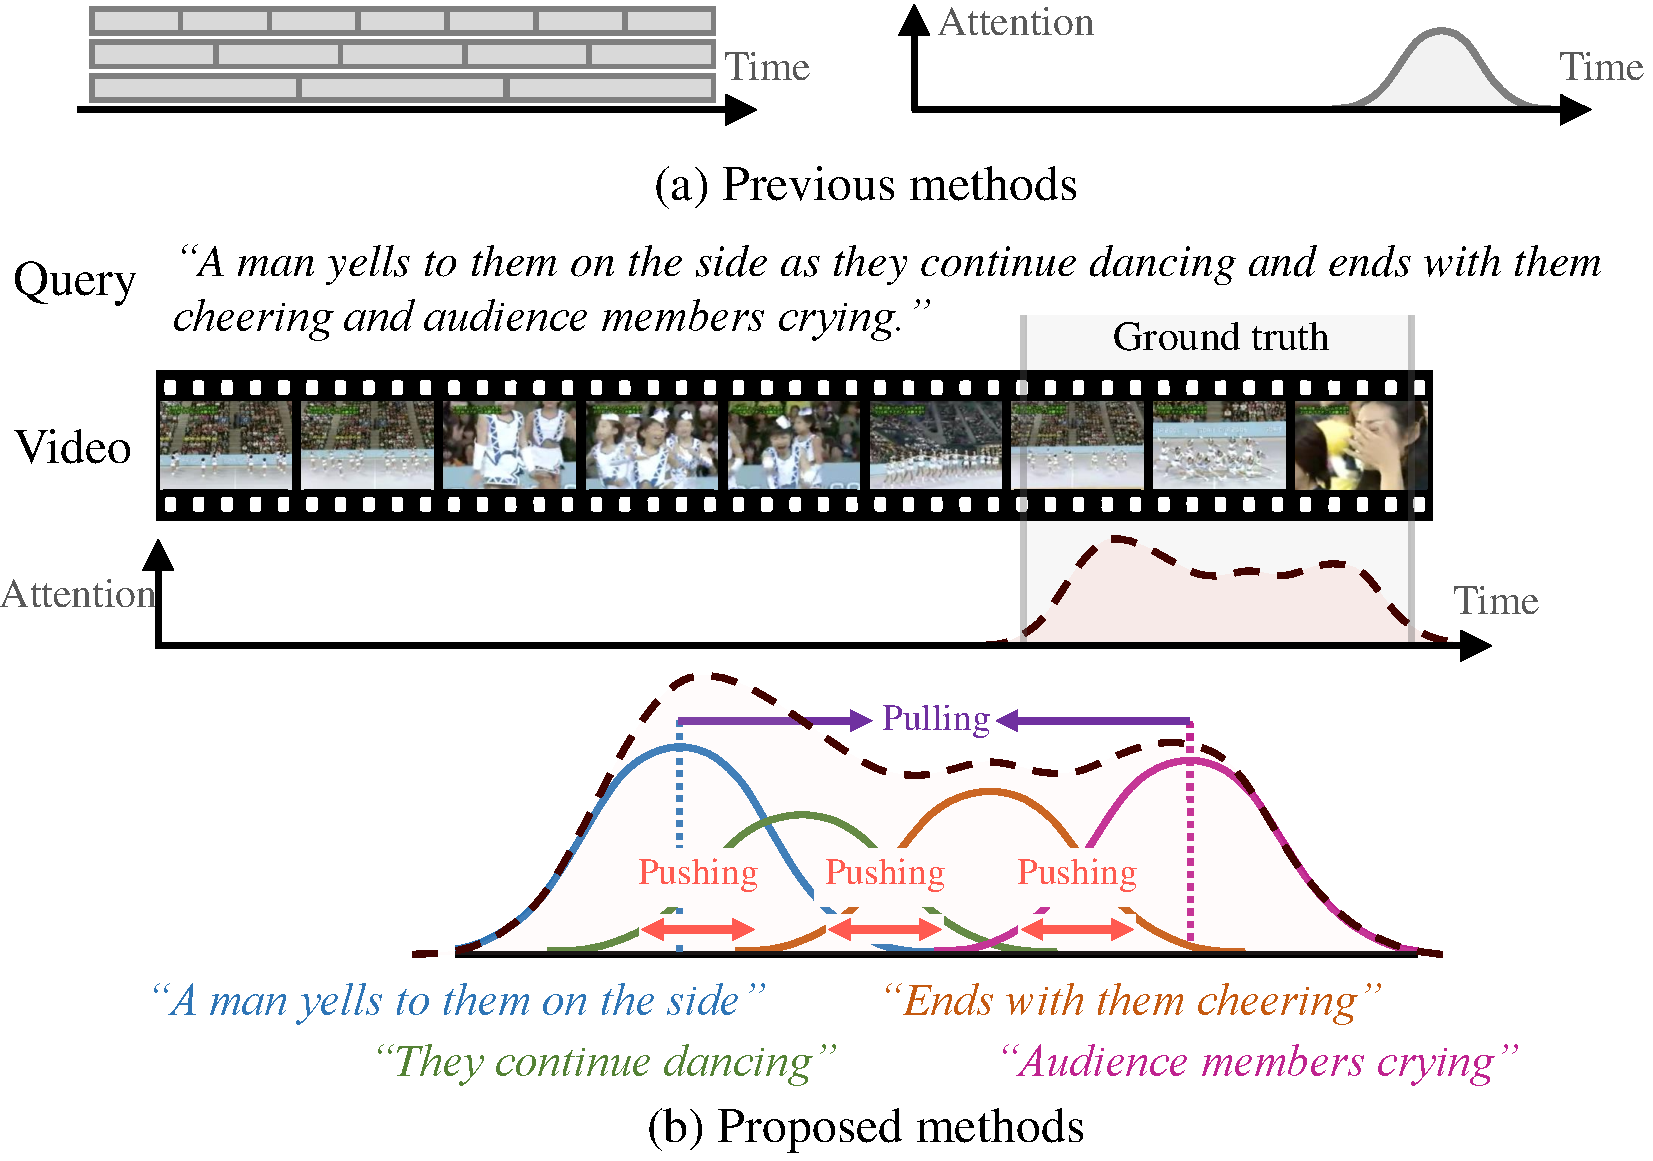
\includegraphics[width=\linewidth]{figures/0-concept-art.pdf}
  \caption{Weakly supervised temporal video grounding. (a) Previous methods use sliding windows (left) or a single Gaussian proposal (right), which has a predetermined shape. (b) The proposed method generates a Gaussian mixture proposal trained to be moderately coupled with a pull-push learning scheme to capture diverse query-relevant events.
  % Further, the proposed method leverages multiple learnable Gaussians for a negative proposal, instead of an existing rule-based one.
  }
\label{fig:concept-art}
\end{figure}

To overcome the limitation, a weakly supervised approach has been proposed to solve the temporal video grounding problem, where only video-sentence pairs are required for training. 
%% Weakly supervised video grounding methods %%%%%%%%%%%%%%%%%%%%%%%%%%%%%%
Some existing methods~\cite{huang2021cross, lin2020weakly, mithun2019weakly, tan2021logan, wang2021weakly, zhang2020counterfactual} use a sliding window strategy to generate proposals for a temporal location but use a lot of pre-defined proposals, which require heavy computation.
%and face difficulties in expressing diverse events described by the sentence query.
%% Gaussian-based methods %%%%%%%%%%%%%%%%%%%%%%%%%%%%%%
To reduce the required number of proposals, \cite{zheng2022cnm, zheng2022cpl} generate learnable Gaussian proposals. 
However, these single Gaussian proposals with a peak at its center lack the expression ability for diverse query-relevant events in a video.

To enhance the expression ability, we propose a Gaussian mixture proposal (GMP) that can depict arbitrary shapes by learning importance, centroid, and range of every Gaussian in the mixture.
% \cite{zong2018deep, lee2018simple}
Since our GMP is implemented over a temporal location, conventional feature-based learning for Gaussian mixture model~\cite{zong2018deep, lee2018simple} is not applicable to our approach.
In our special setting, our goal is to train the GMP to capture a temporal location semantically %relevant to a sentence query.
%We note that a temporal location 
relevant to a sentence query that includes diverse events coupled moderately. %coupled.
In \cref{fig:concept-art}, for instance, one sentence query includes two semantic events coupled by ``A man yells to them on the side" and ``They continue dancing".
%in the given sentence query have their own semantics but are moderately coupled to express one sentence query.

%% Proposed methods %%%%%%%%%%%%%%%%%%%%%%%%%%%%%%
To capture the %moderately 
coupled events in a query, we propose a Pull-Push Scheme (PPS) to learn a GMP whose Gaussians are moderately coupled.
Specifically, we first define a GMP with learnable parameters: importance, centroid, and range of every Gaussian in the mixture.
To learn the importance, we propose an importance weighting strategy that represents importance levels of each Gaussian mask for a query-relevant location.
To generate the GMP that represents a query-relevant location, our PPS is trained to reconstruct the sentence query from the proposal.
In our scheme, the Gaussians in one GMP should be located near a query-relevant temporal location, 
% but should not converge to an identical point to represent diverse events.
but should not be overlapped too much with others to represent diverse events.
To this end, our scheme leverages a pulling loss and a pushing loss, each of which plays an opposite role to the other to produce moderately coupled Gaussians.
The pulling loss lets the Gaussians stay close to each other by pulling the Gaussian centroids together.
% the two farthest masks together.
The pushing loss prevents the Gaussians from overlapping too much with the others by forcing the Gaussians to be less overlapped.

We verify that our scheme generates high-quality proposals that significantly improve recall rates on the Charades-STA~\cite{gao2017tall} and ActivityNet Captions~\cite{krishna2017dense} datasets.
We also demonstrate the effectiveness of each component in our scheme with extensive ablation studies.
%% Contributions %%%%%%%%%%%%%%%%%%%%%%%%%%%%%%
In summary, our contributions are as follows.
\begin{itemize}
\item We generate a Gaussian mixture proposal that represents a query-relevant temporal location by learning importance, centroid, and range of every Gaussian to enhance the expression ability of the proposal.
\item We propose a pull-push learning scheme that uses a pulling loss and a pushing loss, each of which plays an opposite role to the other to capture diverse events.
\item The proposed components are verified in-depth with extensive ablation studies and the overall scheme achieves state-of-the-art performance. 
\end{itemize}
